% !TeX root = ../../latex-talk.tex

\part{SJTUThesis}

\begin{frame}
  \frametitle{简介}
  \begin{columns}
    \begin{column}{0.6\textwidth}
      \begin{itemize}
        \item 最早由韦建文于 2009 年 11 月发布 0.1a 版,2018 年起由 SJTUG 接手维护
        \item 最新版:\SJTUThesisVersion{} (\SJTUThesisDate)
        \item 支持本科、硕士、博士学位论文以及课程论文的排版
      \end{itemize}
    \end{column}
    \begin{column}{0.4\textwidth}
      \begin{exampleblock}{}
        \begin{minipage}[c]{1cm}
          \includegraphics[width=0.8cm]{\getcontribpath{sjtug}{vi/sjtug}}
        \end{minipage}
        \begin{minipage}[c]{2cm}
          \href{https://github.com/sjtug}{sjtug}/\href{https://github.com/sjtug/SJTUThesis}{SJTUThesis}
        \end{minipage}
      \end{exampleblock}
      \vspace{-8pt}
      \begin{block}{}
        \scriptsize
        上海交通大学 \hologo{XeLaTeX} 学位论文及课程论文模板 | Shanghai Jiao Tong University \hologo{XeLaTeX} Thesis Template
      \end{block}
      \vspace{-8pt}
      \begin{alertblock}{}
        \scriptsize
        \begin{tabular}{cl}
          \faStar & 2.4k \\
          \faEye & 55 \\
          \faCodeBranch & 701 \\
        \end{tabular}
      \end{alertblock}
    \end{column}
  \end{columns}
\end{frame}

\begin{frame}
  \frametitle{下载与编译}
  \alert{下载} 推荐安装 Git \link{https://git-scm.com/} 后,克隆 SJTUG 镜像仓库
  \begin{exampleblock}{\faGit*}
    \ttfamily\small
    git clone https://mirror.sjtu.edu.cn/git/SJTUThesis.git/
  \end{exampleblock}

  \alert{编译} 推荐使用 \pkg{latexmk} 编译\footnote{\hologo{MiKTeX} 用户需要手动安装 Perl 解释器 \link{https://www.perl.org/get.html} 才能使用 \pkg{latexmk}。},在不能够利用自带的 \texttt{.latexmkrc} 配置文件的情况下,需要查清楚在对应的编辑器中如何使用 \hologo{XeLaTeX} + \hologo{biber} 编译 \link{https://github.com/sjtug/SJTUThesis/blob/master/README.md}。
  \begin{exampleblock}{\faTerminal}
    \ttfamily\small
    latexmk -xelatex main
  \end{exampleblock}

  Overleaf 用户可以下载压缩包后,上传并采用 \hologo{XeLaTeX} 编译方式。
\end{frame}

\begin{frame}
  \frametitle{手动编译}
  \alert{第一次编译失败} 如果没有办法通过通常方式编译成功,请尝试使用文件夹内附带 \faLinux{}\,\faApple{} \texttt{Makefile} 和 \faWindows{} \texttt{Compile.bat} 进行编译。

  \alert{统计字数} 编写过程中也可以使用对应的命令调用 \TeX{}count 来统计正文字数。
  \begin{columns}
    \begin{column}{0.38\textwidth}
      \begin{exampleblock}{\faLinux{}\,\faApple}
        \ttfamily
        make all\\
        make clean\\
        make cleanall\\
        make wordcount
      \end{exampleblock}
    \end{column}
    \begin{column}{0.38\textwidth}
      \begin{exampleblock}{\faWindows}
        \ttfamily
        ./Compile.bat thesis\\
        ./Compile.bat clean\\
        ./Compile.bat cleanall\\
        ./Compile.bat wordcount
      \end{exampleblock}
    \end{column}
    \begin{column}{0.24\textwidth}
      \begin{block}{\faInfo}
        \ttfamily
        编译论文\\
        清理中间文件\\
        $\hookrightarrow +$删除论文\\
        统计字数
      \end{block}
    \end{column}
  \end{columns}
\end{frame}

\begin{frame}[label=compile]
  \frametitle{编译问题排查}
  \begin{columns}
    \begin{column}{0.33\textwidth}
      \begin{alertblock}{无法使用 \texttt{latexmk}\thesisissue{578}}
        \hologo{MiKTeX} 需要安装 Perl 解释器。
      \end{alertblock}  
      \begin{alertblock}{C\TeX{} 套装无法编译\thesisissue{446}}
        使用最新 \TeX{} 发行版。
      \end{alertblock}
      \begin{alertblock}{\hologo{pdfLaTeX} 无法编译\thesisissue{444}}
        请使用 \texttt{latexmk},或更改编辑器设置以 \hologo{XeLaTeX} 编译。
      \end{alertblock}
    \end{column}
    \begin{column}{0.33\textwidth}
      \begin{alertblock}{缺少字体\thesisissue{564} \thesisdiscuss{598}}
        更换字体集,或者安装对应字体。
      \end{alertblock}
      \begin{alertblock}{缺少汉字\thesisissue{533} \thesisdiscuss{617}}
        去除使用 fandol 字体集的设定。或者是安装字体后,改用 \texttt{fontset=adobe} 或 \texttt{fontset=founder}。
      \end{alertblock}
    \end{column}
    \begin{column}{0.33\textwidth}
      \begin{block}{\faInfoCircle{} README}
        不同编辑器的设置请首先参阅 README \link{https://github.com/sjtug/SJTUThesis/blob/master/README.md} 文档。
      \end{block}
      \begin{block}{\faBookOpen{} Wiki}
        其他编译问题推荐查阅 Wiki \link{https://github.com/sjtug/SJTUThesis/wiki} 的使用说明部分。
      \end{block}
    \end{column}
  \end{columns}
\end{frame}

\begin{frame}[fragile, label=covers]
  \begin{codeblock}[firstnumber=3]{main.tex}
|\alert{\% 载入 SJTUThesis 模版}|
\documentclass[|\only<1>{\highlight{type}}\only<2>{type}|=|\only<1>{bachelor}\only<2>{\highlight{bachelor}}|]{sjtuthesis}
  \end{codeblock}
  \begin{figure}
    \parbox{0.9\textwidth}{
      \begin{subfigure}{0.20\textwidth}
        \framebox{\includegraphics[width=\linewidth]{support/thesis/bachelor}}
        \caption{\only<1>{学士}\only<2>{\texttt{bachelor}}}
      \end{subfigure}\hfill
      \begin{subfigure}{0.20\textwidth}
        \framebox{\includegraphics[width=\linewidth]{support/thesis/master}}
        \caption{\only<1>{硕士}\only<2>{\texttt{master}}}
      \end{subfigure}\hfill
      \begin{subfigure}{0.20\textwidth}
        \framebox{\includegraphics[width=\linewidth]{support/thesis/doctor}}
        \caption{\only<1>{博士}\only<2>{\texttt{doctor}}}
      \end{subfigure}\hfill
      \begin{subfigure}{0.20\textwidth}
        \framebox{\includegraphics[width=\linewidth]{support/thesis/course}}
        \caption{\only<1>{课程}\only<2>{\texttt{course}}}
      \end{subfigure}
      \caption{论文类型示例\only<2>{ \texttt{type}}}
    }
  \end{figure}
\end{frame}

\begin{frame}[fragile]
  \frametitle{文档类选项}
  % \framesubtitle{\textbackslash{}documentclass\{sjtuthesis\}}
  \begin{columns}
    \begin{column}{0.4\textwidth}
      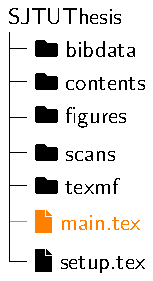
\includegraphics[page=1]{thesisdir}
    \end{column}
    \begin{column}{0.6\textwidth}
      \begin{table}[H]
        \caption{文档类选项}
        \footnotesize
        \begin{tabular}{>{\ttfamily}rll}
          \toprule
          选项 & 含义 & 相关 \\
          \midrule
          type= & 指定论文类型 & 第 \ref{covers} 页\\
          fontset= & 指定字体 & 第 \ref{compile} 页\\
          \midrule
          review & 开启盲审模式 & \thesisissue{195} \thesisissue{686} \\
          twoside & 双页模式 & \thesisissue{554} \\
          oneside & 单页模式 & \thesisissue{694} \\
          openright & 章从奇数页开始 & \thesisdiscuss{724} \\
          openany & 章从任意页开始 & \thesisissue{446} \\
          \bottomrule
        \end{tabular}
      \end{table}
    \end{column}
  \end{columns}
\end{frame}

\begin{frame}[fragile]
  \frametitle{基本配置}
  \framesubtitle{\textbackslash{}input\{setup\}}
  \begin{columns}
    \begin{column}{0.35\textwidth}
      \includegraphics[page=2]{thesisdir}
    \end{column}
    \begin{column}{0.65\textwidth}
      \begin{codeblock}[firstnumber=12]{main.tex}
|\highlightline<1>|% 论文基本配置,加载宏包等全局配置
|\highlightline<1>|% !TEX root = ./main.tex

\sjtusetup{
  %
  %******************************
  % 注意:
  %   1. 配置里面不要出现空行
  %   2. 不需要的配置信息可以删除
  %******************************
  %
  % 信息录入
  %
  info = {%
    %
    % 标题
    %
    title           = {上海交通大学学位论文 \LaTeX{} 模板示例文档},
    title*          = {A Sample Document for \LaTeX-based SJTU Thesis Template},
    %
    % 标题页标题
    %   可使用“\\”命令手动控制换行
    %
    % display-title   = {上海交通大学学位论文\\ \LaTeX{} 模板示例文档},
    % display-title*  = {A Sample Document \\ for \LaTeX-based SJTU Thesis Template},
    %
    % 页眉标题
    %
    % running-title   = {示例文档},
    % running-title*  = {Sample Document},
    %
    % 关键词
    %
    keywords        = {上海交大, 饮水思源, 爱国荣校},
    keywords*       = {SJTU, master thesis, XeTeX/LaTeX template},
    %
    % 姓名
    %
    author          = {某\quad{}某},
    author*         = {Mo Mo},
    %
    % 指导教师
    %
    supervisor      = {某某教授},
    supervisor*     = {Prof. Mou Mou},
    %
    % 副指导教师
    %
    % assisupervisor  = {某某教授},
    % assisupervisor* = {Prof. Uom Uom},
    %
    % 学号
    %
    id              = {0010900990},
    %
    % 学位
    %   本科生不需要填写
    %
    degree          = {工学硕士},
    degree*         = {Master of Engineering},
    %
    % 专业
    %
    major           = {某某专业},
    major*          = {A Very Important Major},
    %
    % 所属院系
    %
    department      = {某某系},
    department*     = {Depart of XXX},
    %
    % 课程名称
    %   仅课程论文适用
    %
    course          = {某某课程},
    %
    % 答辩日期
    %   使用 ISO 格式 (yyyy-mm-dd);默认为当前时间
    %
    % date            = {2014-12-17},
    %
    % 资助基金
    %
    % fund  = {
    %           {国家 973 项目 (No. 2025CB000000)},
    %           {国家自然科学基金 (No. 81120250000)},
    %         },
    % fund* = {
    %           {National Basic Research Program of China (Grant No. 2025CB000000)},
    %           {National Natural Science Foundation of China (Grant No. 81120250000)},
    %         },
  },
  %
  % 风格设置
  %
  style = {%
    %
    % 本科论文页眉 logo 颜色 (red/blue/black)
    %
    % header-logo-color = black,
  },
  %
  % 名称设置
  %
  name = {
    % bib               = {References},
    % acknowledgements  = {谢\hspace{\ccwd}辞},
    % publications      = {攻读学位期间完成的论文},
  },
}

% 使用 BibLaTeX 处理参考文献
%   biblatex-gb7714-2015 常用选项
%     gbnamefmt=lowercase     姓名大小写由输入信息确定
%     gbpub=false             禁用出版信息缺失处理
\usepackage[backend=biber,style=gb7714-2015]{biblatex}
% 文献表字体
% \renewcommand{\bibfont}{\zihao{-5}}
% 文献表条目间的间距
\setlength{\bibitemsep}{0pt}
% 导入参考文献数据库
\addbibresource{bibdata/thesis.bib}

% 定义图片文件目录与扩展名
\graphicspath{{figures/}}
\DeclareGraphicsExtensions{.pdf,.eps,.png,.jpg,.jpeg}

% 确定浮动对象的位置,可以使用 [H],强制将浮动对象放到这里(可能效果很差)
% \usepackage{float}

% 固定宽度的表格
% \usepackage{tabularx}

% 使用三线表:toprule,midrule,bottomrule。
\usepackage{booktabs}

% 表格中支持跨行
\usepackage{multirow}

% 表格中数字按小数点对齐
\usepackage{dcolumn}
\newcolumntype{d}[1]{D{.}{.}{#1}}

% 使用长表格
\usepackage{longtable}

% 附带脚注的表格
\usepackage{threeparttable}

% 附带脚注的长表格
\usepackage{threeparttablex}

% 算法环境宏包
\usepackage[ruled,vlined,linesnumbered]{algorithm2e}
% \usepackage{algorithm, algorithmicx, algpseudocode}

% 代码环境宏包
\usepackage{listings}
\lstnewenvironment{codeblock}[1][]%
  {\lstset{style=lstStyleCode,#1}}{}

% 物理科学和技术中使用的数学符号,定义了 \qty 命令,与 siunitx 3.0 有冲突
% \usepackage{physics}

% 直立体数学符号
\newcommand{\dd}{\mathop{}\!\mathrm{d}}
\newcommand{\ee}{\mathrm{e}}
\newcommand{\ii}{\mathrm{i}}
\newcommand{\jj}{\mathrm{j}}

% 国际单位制宏包
\usepackage{siunitx}[=v2]

% 定理环境宏包
\usepackage{ntheorem}
% \usepackage{amsthm}

% 绘图宏包
\usepackage{tikz}
\usetikzlibrary{shapes.geometric, arrows}

% 一些文档中用到的 logo
\usepackage{hologo}
\newcommand{\XeTeX}{\hologo{XeTeX}}
\newcommand{\BibLaTeX}{\textsc{Bib}\LaTeX}

% 借用 ltxdoc 里面的几个命令方便写文档
\DeclareRobustCommand\cs[1]{\texttt{\char`\\#1}}
\providecommand\pkg[1]{{\sffamily#1}}

% 自定义命令

% E-mail
\newcommand{\email}[1]{\href{mailto:#1}{\texttt{#1}}}

% hyperref 宏包在最后调用
\usepackage{hyperref}

% 自动引用题注更正为中文
\def\equationautorefname{式}
\def\footnoteautorefname{脚注}
\def\itemautorefname{项}
\def\figureautorefname{图}
\def\tableautorefname{表}
\def\partautorefname{篇}
\def\appendixautorefname{附录}
\def\chapterautorefname{章}
\def\sectionautorefname{节}
\def\subsectionautorefname{小节}
\def\subsubsectionautorefname{小节}
\def\paragraphautorefname{段落}
\def\subparagraphautorefname{子段落}
\def\FancyVerbLineautorefname{行}
\def\theoremautorefname{定理}


\begin{document}

%TC:ignore

|\highlightline<2>|% 标题页
|\highlightline<2>|\maketitle
\end{codeblock}
\visible<2>{
  \cmd{sjtusetup} 中的 \pkg{info} 将会修改封面的信息设置(见第 \ref{covers} 页)。
}
\end{column}
\end{columns}
\end{frame}

\begin{frame}[fragile]
  \frametitle{基本配置}
  \framesubtitle{\textbackslash{}sjtusetup}
  \begin{columns}
    \begin{column}{0.35\textwidth}
      \includegraphics[page=3]{thesisdir}
    \end{column}
    \begin{column}{0.65\textwidth}
      \begin{codeblock}[firstnumber=3]{setup.tex}
\sjtusetup{
  info = {
    title    = {||上海交通大学学位论文 \LaTeX{} 模板示例文档},
    title*   = {A Sample for \LaTeX-based SJTU Thesis Template},
    author   = {||某\quad{}某},
    author* = {Mo Mo},
  },
  style = { header-logo-color = red,
  },
  name = {
    publications = {||攻读学位期间完成的论文},
  },
}
      \end{codeblock}
    \end{column}
  \end{columns}
\end{frame}

\begin{frame}
  \frametitle{基本配置}
  \framesubtitle{\textbackslash{}sjtusetup}
  \begin{columns}
    \begin{column}{0.35\textwidth}
      \includegraphics[page=3]{thesisdir}
    \end{column}
    \begin{column}{0.65\textwidth}
      \begin{table}[H]
        \centering
        \caption{info 域}
        \footnotesize
        \begin{tabular}{lll} \toprule
          命令作用     & 中文对应选项                      & 英文对应选项             \\ \midrule
          论文标题     & \texttt{title}                    & \texttt{title*}          \\
          关键字列表   & \texttt{keywords}                 & \texttt{keywords*}       \\
          作者姓名     & \texttt{author}                   & \texttt{author*}         \\
          申请学位名称 & \texttt{degree}                   & \texttt{degree*}         \\
          院系名称     & \texttt{department}               & \texttt{department*}     \\
          专业名称     & \texttt{major}                    & \texttt{major*}          \\
          导师         & \texttt{supervisor}               & \texttt{supervisor*}     \\
          副导师       & \texttt{assisupervisor}           & \texttt{assisupervisor*} \\
          日期         & \multicolumn{2}{c}{\texttt{date}}                            \\
          学号         & \multicolumn{2}{c}{\texttt{id}}                              \\ \bottomrule
        \end{tabular}
      \end{table}
    \end{column}
  \end{columns}
\end{frame}

\begin{frame}[fragile]
  \frametitle{版权页}
  \framesubtitle{\textbackslash{}copyrightpage}
  \begin{columns}
    \begin{column}{0.4\textwidth}
      \only<1>{
        \includegraphics[page=2]{thesisdir}
      }
      \only<2>{
        \includegraphics[page=4]{thesisdir}
      }
      \only<3>{
        \begin{figure}[H]
          \framebox{\includegraphics[page=2,width=0.4\linewidth]{bachelor}}
          \caption{版权页}
        \end{figure}
      }
    \end{column}
    \begin{column}{0.6\textwidth}
      \begin{codeblock}[firstnumber=22]{main.tex}
|\highlightline<1>|% 原创性声明及使用授权书
|\highlightline<1>|\copyrightpage
|\highlightline<2>|% 插入外置原创性声明及使用授权书
|\highlightline<2>|% \copyrightpage[scans/sample-copyright-old.pdf]
      \end{codeblock}
      \only<1>{
        \cmd{copyrightpages} 可以用于插入版权页。
      }
      \only<2>{
        \cmd{copyrightpages} 也接受一个可选参数,用于直接使用扫描件。\thesisissue{473}
      }
      \only<3>{
        现在原创性声明与使用授权书已合并为一页。
      }
    \end{column}
  \end{columns}
\end{frame}

\begin{frame}
  \frametitle{数学}
  \begin{columns}
    \begin{column}{0.4\textwidth}
      \includegraphics[page=5]{thesisdir}
    \end{column}
    \begin{column}{0.6\textwidth}
      \SJTUThesis{} 定义了常用的数学环境(需要引入 \pkg{ntheorem} 或者 \pkg{amsthm} 宏包)。

      \begin{table}[H]
        \centering
        \caption{\textsc{SJTUThesis} 定义的数学环境}
        \footnotesize
        \begin{tabular}{>{\ttfamily}rl|>{\ttfamily}rl}
          \toprule
          assumption  & 假设  & lemma       & 引理 \\
          axiom       & 公理  & problem     & 问题 \\
          conjecture  & 猜想  & proof       & 证明 \\
          corollary   & 推论  & proposition & 命题 \\
          definition  & 定义  & remark      & 注   \\
          example     & 例    & solution    & 解   \\
          exercise    & 练习  & theorem     & 定理 \\
          \bottomrule
        \end{tabular}
      \end{table}

      \SJTUThesis{} 可以通过 \texttt{unimath} 选项使用 \pkg{unicode-math} 进行数学输入,注意与传统方式的区别。\thesisissue{555}
    \end{column}
  \end{columns}
\end{frame}

\begin{frame}[fragile]
  \frametitle{参考文献}
  \begin{columns}
    \begin{column}{0.4\textwidth}
      \includegraphics[page=6]{thesisdir}
    \end{column}
    \begin{column}{0.6\textwidth}
      \begin{codeblock}[firstnumber=111,numbersep=2pt]{setup.tex}
% 使用 BibLaTeX 处理参考文献
%   biblatex-gb7714-2015 常用选项
%     gbnamefmt=lowercase     姓名大小写由输入信息确定
%     gbpub=false             禁用出版信息缺失处理
\usepackage[backend=biber,style=gb7714-2015]{biblatex}
% 文献表字体
% \renewcommand{\bibfont}{\zihao{-5}}
% 文献表条目间的间距
\setlength{\bibitemsep}{0pt}
|\highlightline|% 导入参考文献数据库
|\highlightline|\addbibresource{bibdata/thesis.bib}
      \end{codeblock}
    \end{column}
  \end{columns}
\end{frame}

\begin{frame}
  \frametitle{还有其他问题?}
  \begin{columns}
    \begin{column}{0.73\textwidth}
      \begin{itemize}
        \item[{\faComment*[regular]}] 日常模板或 \LaTeX{} 使用问题可以前往 Discussions \link{https://github.com/sjtug/SJTUThesis/discussions} 提问

        (解决后别忘了 \textcolor{green}{\faCheckCircle{} Mark as answer}
        \item[{\faDotCircle[regular]}] 如果是 \textsc{SJTUThesis} 项目本身的 bug 和 feature request

        可以通过 Issues \link{https://github.com/sjtug/SJTUThesis/issues} 反馈。
        \item[{\faCodeBranch}] 如果你有好点子,可以贡献代码

          向 \textsc{SJTU\TeX{}}(v1) \link{https://github.com/sjtug/SJTUTeX/tree/v1} 存储库发 PR,\par
          而后把解包结果同步到 \textsc{SJTUThesis}。

        \item[{\faTag}] 如果你对正在基于 \LaTeX3 开发的新版感兴趣,\par
          也欢迎向 \textsc{SJTU\TeX{}}(v2) \link{https://github.com/sjtug/SJTUTeX/tree/v2} 发 PR。

        \item[{\faQq}] 也欢迎在 QQ 群即时讨论。
      \end{itemize}
    \end{column}
    \begin{column}{0.27\textwidth}
      
\includegraphics[height=0.7\textheight]{qq.jpg}
    \end{column}
  \end{columns}
\end{frame}